\section{Machines}\label{sec:contribs:machines}

du texte

\subsection{idchire}\label{sec:contribs:machines:idchire}
Encore du texte

\begin{figure}[ht]
  \centering
  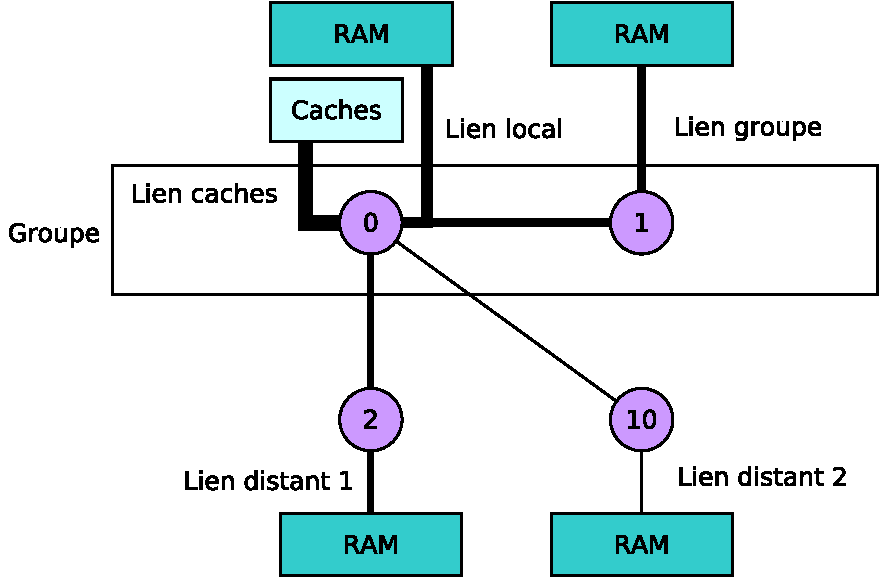
\includegraphics[width=\textwidth]{topo-idchire}
  \caption{Topologie schématique vu du nœud 0}\label{fig:contribs:machines:idchire:topo-liens}
\end{figure}

\begin{figure}[ht]
  \centering
  \includegraphics[width=\textwidth]{heatmap_idchire_memcpy}
  \caption{Carte de la bande passante d'idchire}\label{fig:contribs:machines:idchire:heatmap}
\end{figure}

\begin{todo}
  Figure saturation lien local
\end{todo}

\begin{todo}
  Figure saturation output du noeud
\end{todo}

\subsection{brunch}\label{sec:contribs:machines:brunch}

